%\newpage
  \begin{titlepage}
    \vspace*{\fill}
      \part{Introduction}
    \vspace*{\fill}
  \end{titlepage}

%\chapter{Introduction}\label{ch:introduction}
\phantomsection
\chapter*{Contents}

First, this project is motivated by analyzing the need of robust facial expression recognition systems for various applications. Then already existing algorithms will be studied to choose one that is basic but effective in order to improve it. In the last part, the problem will be formulated.
\pagebreak

\phantomsection
\chapter{Motivation}

A facial expression is a visible manifestation of the effective state, cognitive activity, intent, personality, and psychopathology of a person \cite{DON99}; facial expressions play a significant role in human dialogue and interaction. Indeed, facial expressions carry more informations than mere speech, informations on which humans can relay for interaction. Facial expressions have a considerable effect on a listening interlocutor; a speaker facial expressions accounts for about 55 percent of the effect, 38 percent of the latter is conveyed by voice intonation and 7 percent by the spoken words \cite{PAN00}.
\newline

\noindent Since Antiquity, researchers have been interested in emotion and more particularly in emotion recognition. But one of the important studies on facial expression analysis impacting on the modern day science of automatic facial expression recognition was the work carried out by Charles Darwin \cite{BET12}. In 1872, Darwin wrote a treatise that established general expression principles and expression means for both humans and animals \cite{DAR04}. He also classified various kinds of expressions. This can be considered as the beginning of facial expression recognition.
\newline

\noindent Now, with the emergence of new technologies and computers, research is now focused on computer-based automatic facial expression recognition. Because facial expressions are major factors in human interaction, this research field will broaden the domain of Human-Machine Interaction. Indeed, emotion recognition will enable computers to be more responsive to users' emotions, and allow interactions to become more and more realistic. 
\newline

\noindent Another domain where facial expression recognition is an important issue is robotics. With the advances made in robotics, robots nowadays tend to mimic human emotion and react as as human-like as possible, especially for humanoid robots. However, since robots are being more and more present in our daily lives, they need to understand and recognize human emotions.
\newline

\noindent There are also various other domains where emotion recognition can be used: Telecommunications, behavioral science, video games, animations, psychiatry, automobile safety, affect-sensitive music juke boxes and televisions, educational software, etc \cite{BET12}.
\newline

\noindent A lot of real time applications have already been created. For example, Bartlett et al. have successfully used their face expression recognition system to develop an animated character that mirrors the expressions of the user (called CU Animate) \cite{BAR03}. They have also been successful in deploying the recognition system on Sony's Aibo Robot and ATR's RoboVie \cite{BAR03}. Another interesting application has been demonstrated by Anderson and McOwen, called "EmotiChat" \cite{AND06}. It is a regular chatroom, except the fact that their facial expression recognition system is connected to the chat and convert the users' facial expressions into emoticons. Because facial expression recognition systems' robustness and reliability are constantly increasing, lots of innovative applications will appear.
\newpage

\phantomsection
\chapter{Facial expression recognition}

\phantomsection
\section{General structure}

\noindent Facial Expression Recognition is a system that allows to recognize emotion on a human face in an automatic way. Facial Expression Recognition can be based on images or on videos; it can be real time or not. Most of the time, searchers use images of human faces and try to recognize the emotion. But this can also be done in real time by using video. While the person is having and expressing his emotions, the Facial Expression Recognition system is analyzing the video and detect in real time the emotion of the person.
\newline

\noindent In both cases, Facial Expression Recognition process is composed as follows:


\noindent 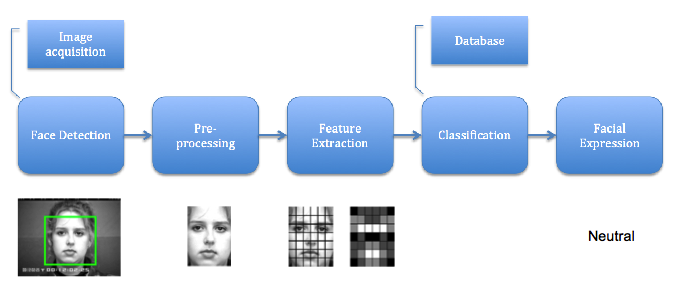
\includegraphics[scale=0.6]{figures/facial_expression_recognition_process}

\noindent The first step of the process is "Image Acquisition". The images used for Facial Expression Recognition can be static images or a image sequences. Image sequences gives more information about the facial expression, as the steps in the movement of the muscles of the face to get to the facial expression. Concerning the static images, most of the time, 2D grey-scale images are used for automatic Facial Expression Recognition system. But in the future, more and more systems will potentially use more and more colour images. First because the technologies capable of capturing images or image sequences become more affordable. And then, because colours can give more information on emotion as blushing \cite{CHI03}.
\newline

\noindent The second step is "Face Detection". "Face Detection" is a step that can be included in the 'Pre-processing' one. But because it is necessary to do it; it represents a step in itself. Indeed, in a static image and even more in an image sequence, the need of detecting the face is obvious. Once the face has been detecting, all the other information in the image can be deleted; only the face is needed. In a Facial Expression Recognition system working in real-time with image sequences, the face needs to be detected but also to be tracked. The most used and famous algorithm capable of doing that is the Viola-Jones Algorithm. It can be trained to detect all kind of objects; but it is mostly used for face detection.
\newline

\noindent The third step is "Pre-processing". It consists of applying different processing to the image. This way the image processed is optimized for the next step that is "Features Extraction".The most used processing are: noise removal, normalization against the variation of pixel position or brightness, segmentation, location, or tracking of the parts of the face. Emotion recognition is also sensitive to transformation, scaling and rotation of the head in the image or image sequence. In order to supplant this problem, the image can be geometrically standardized. Usually, this standardization is based on references that make the eyes \cite{CHI03}.
\newline

\noindent Once the image has been prepared while the "Pre-processing" part, the next and fourth step is "Features Extraction". It is this step that converts image data into a higher representation of shape, texture, color, etc... The extracted data are used for the next step that is "Classification". One of the main goals of this step is to reduce the dimensionality of the input space. The reduction procedure should retain essential information possessing high discrimination power and high stability \cite{CHI03}. There is a lot of features extraction methods. The most famous are : Principal Component Analysis (PCA), Linear Discriminant Analysis (LDA), Problem Based Learning (PBL), Hidden Markov Model (HMM), Eigenfaces, Gabor Wavelets.
\newline

\phantomsection
\section{Existing systems}

\noindent Principal Component Analysis (PCA) : Principal Component Analysis is a statistical method; one of the most used in linear algebra. PCA is mainly used to reduce high dimensionality of data and to obtain the most important information from this data. Because Facial Expression Recognition needs to reduce the dimensionality of data during features extraction, PCA is commonly used. It helps transforming high dimensionality of data to a new coordinate system of lower dimensions while still preserving the most important information. PCA computes a covariance matrix and a set of values called the eigenvalues and eigenvectors from the original data \cite{GAN08}.
\newline

\noindent Linear Discriminant Analysis (LDA) : Linear Discriminant Analysis is a statistical method as PCA, used to classify a set of objects into groups. It is done by observing a set of features that describe the objects. LDA as PCA are used to establish a linear relationship between the dimensions of the data. The main difference is that LDA uses the linear relationship to model the differences into classes of objects and PCA does not take any differences into account in the linear relationship. The idea is to perform a linear transformation on the data to obtain a lower dimensional set of features \cite{GAN08}.
\newline

\noindent Problem Based Learning (PBL) : Problem Based Learning is a features extraction method with an appearance based approach. It can be used to describe texture and shape. PBL extracts some informations from the neighborhood of a central pixel. It compares the intensity values of the neighborhood pixels with the intensity value of the central pixel  \cite{GAN08}.
\newline

\noindent Hidden Markov Model (HMM)
\newline
\noindent Eigenfaces
\newline
\noindent Gabor Wavelets
\newline

\phantomsection
\section{Issues}

\noindent bla bla bla
\newline

\phantomsection
\section{Requirements}

\noindent bla bla bla
\newline









\noindent Before developing a facial expression recognition project, it is important to know what already exist; the state of the art of facial expression recognition system. In this chapter, an overview will be given of the existing systems before to decide on a system for the project.
\newline
